\documentclass[10pt]{beamer}

% \usepackage{define}
\usepackage{animate}

\usetheme{CCFD}
\usepackage{color}
\definecolor{gray97}{gray}{.90}
\definecolor{gray75}{gray}{.75}
\usepackage{listings}
\lstset{frame=Ltb,
     framerule=0pt,
     aboveskip=0cm,
     framextopmargin=0pt,
     framexbottommargin=0pt,
     framexleftmargin=0cm,
     framesep=0pt,
     rulesep=0pt,
     backgroundcolor=\color{gray97},
     rulesepcolor=\color{black},
     language=C,
           basicstyle=\ttfamily\scriptsize,
           keywordstyle=\color{blue}\ttfamily,
           stringstyle=\color{red}\ttfamily,
           commentstyle=\color{green}\ttfamily,
          breaklines=true,
          }
\lstdefinestyle{consol}
   {basicstyle=\scriptsize\bf\ttfamily,
    backgroundcolor=\color{gray75},
}
\resetcounteronoverlays{lstnumber}

\newcommand{\tabitem}{%
  \usebeamertemplate{itemize item}\hspace*{\labelsep}}

\usepackage{tikz}
\usetikzlibrary{calc,shapes,arrows.meta}

\eventtitle{Computer Science I}
\title{Lecture 7\\1D Arrays}
\date{}

\setbeamertemplate{blocks}[rounded][shadow=true]
\setbeamertemplate{navigation symbols}[]

\newcommand\aeDiagonalNumber{100}
\newcommand\memorySixtyFive{%%' 
  \begin{minipage}{2.75cm}
    \centering
    char `a' in memory\par       
    (65 = ascii code)
  \end{minipage}}

\begin{document}

\frame{
    \titlepage
}

\section{Today}
\begin{frame}
  \frametitle{Today}
  \framesubtitle{Fun as always {\tiny at least for some}}
  \begin{itemize}
    \item How to create 1D static arrays
    \item How do arrays compare to pointers
    \item Some (strange) consequences of pointer arithmetic
    \item Functions, and passing arrays to functions
    \item Basic sorting algorithms - bubble sort
    \item Generating random numbers
    \item Input output operatios on files
    \item Examples
  \end{itemize}
\end{frame}

\section{1D arrays}

\begin{frame}[fragile]
  \frametitle{1D arrays}
  \framesubtitle{Declaration and memory}
  \vspace{-0.3cm}
  \begin{columns}
    \begin{column}{0.65\textwidth}
      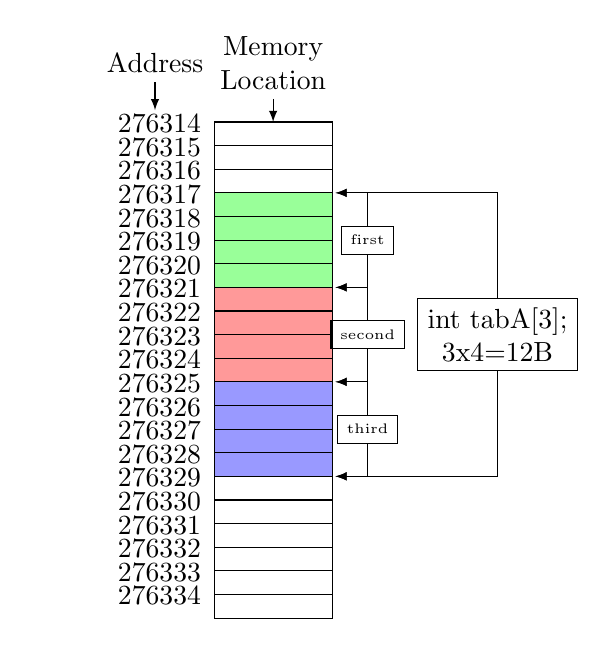
\begin{tikzpicture}[x=1.5cm,y=0.3cm]
  %% Building the boxes representing memory locations
  \foreach \x in {0,1,...,20}
  {
    \node[inner sep=1pt] (BL\x) at (0,-\x)   {};
    \node[inner sep=1pt] (UR\x) at (1,-\x+1) {};
    \node (MM\x) at ($(BL\x)!0.5!(UR\x)$) {};
    \draw (BL\x) rectangle (UR\x);
    \edef\memoryNumber{\number\numexpr276314+\x\relax}
    \node[anchor=south east] at (BL\x.north west) {\memoryNumber};
  }

  %% Label columns:
  \node (MEMLOC) at ($(MM0)+(0.0,0.9cm)$) { \parbox{2cm}{\centering Memory Location} };
  \node (ADDRESS) at ($(MEMLOC)-(1.0,0)$) {\parbox{3cm}{\centering Address} };
  \draw [-latex] (MEMLOC) -- ($(MM0|-UR0)+(0.0,0)$);
  \draw [-latex] (ADDRESS) -- ($(MM0|-UR0)-(1,-0.5)$);

  \foreach \x in {3,...,6}
  {
    \node[inner sep=1pt] (BL\x) at (0,-\x)   {};
    \node[inner sep=1pt] (UR\x) at (1,-\x+1) {};
    \node (MM\x) at ($(BL\x)!0.5!(UR\x)$) {};
    \draw[fill=green!40] (BL\x) rectangle (UR\x);
  }
  \foreach \x/\y in {7/3}
  {
    \node[draw] (M\x-\y) at ($0.5*(UR\x)+0.5*(UR\y)+(0.3,0)$)
    { {\centering \tiny first}};
    \draw[-latex]  (M\x-\y) |- (UR\x) ; 
    \draw[-latex]  (M\x-\y) |- (UR\y) ;
  }
  \foreach \x in {7,...,11}
  {
    \node[inner sep=1pt] (BL\x) at (0,-\x)   {};
    \node[inner sep=1pt] (UR\x) at (1,-\x+1) {};
    \node (MM\x) at ($(BL\x)!0.5!(UR\x)$) {};
    \draw[fill=red!40] (BL\x) rectangle (UR\x);
  }
  \foreach \x/\y in {11/7}
  {
    \node[draw] (M\x-\y) at ($0.5*(UR\x)+0.5*(UR\y)+(0.3,0)$)
    { {\centering \tiny second}};
    \draw[-latex]  (M\x-\y) |- (UR\x) ; 
    \draw[-latex]  (M\x-\y) |- (UR\y) ;
  }
  \foreach \x in {11,...,14}
  {
    \node[inner sep=1pt] (BL\x) at (0,-\x)   {};
    \node[inner sep=1pt] (UR\x) at (1,-\x+1) {};
    \node (MM\x) at ($(BL\x)!0.5!(UR\x)$) {};
    \draw[fill=blue!40] (BL\x) rectangle (UR\x);
  }
  \foreach \x/\y in {15/11}
  {
    \node[draw] (M\x-\y) at ($0.5*(UR\x)+0.5*(UR\y)+(0.3,0)$)
    { {\centering \tiny third}};
    \draw[-latex]  (M\x-\y) |- (UR\x) ; 
    \draw[-latex]  (M\x-\y) |- (UR\y) ;
  }
  
  \foreach \x/\y in {15/3}
  {
    \node[draw] (M\x-\y) at ($0.5*(UR\x)+0.5*(UR\y)+(1.4,0)$)
    { \parbox{1.8cm}{\centering int tabA[3];\\3x4=12B}};
    \draw[-latex]  (M\x-\y) |- (UR\x) ; 
    \draw[-latex]  (M\x-\y) |- (UR\y) ;
  }


\end{tikzpicture}
    \end{column}
    \begin{column}{0.5\textwidth}
Syntax:
\begin{lstlisting}
type name[size]
\end{lstlisting}
\begin{itemize}
  \item \textit{type} - almost any type, pointer, etc.
  \item \textit{name} - an identifier
  \item \textit{size} - \textbf{MUST} be known at compilation time 
\end{itemize}
e.g.:
\begin{lstlisting}
//Array of 3 ints
int tabA[3];
//array of 5 doubles
double tabB[5];
\end{lstlisting}
\begin{itemize}
  \item Continous in memory
  \item Occupies \textit{size} x \textit{sizeof(type)} B
\end{itemize}
    \end{column}
  \end{columns}
\end{frame}

\begin{frame}[fragile]
  \frametitle{1D arrays}
  \framesubtitle{The size \textbf{MUST} be known}
  You will lose points if you do:
\begin{lstlisting}
int n=8;
int tabA[n];
scanf("%d",&n);
double tabA[n];
\end{lstlisting}
\end{frame}

\begin{frame}[fragile]
  \frametitle{1D arrays}
  \framesubtitle{Acces to elements}
  \vspace{-0.3cm}
  \begin{columns}
    \begin{column}{0.65\textwidth}
      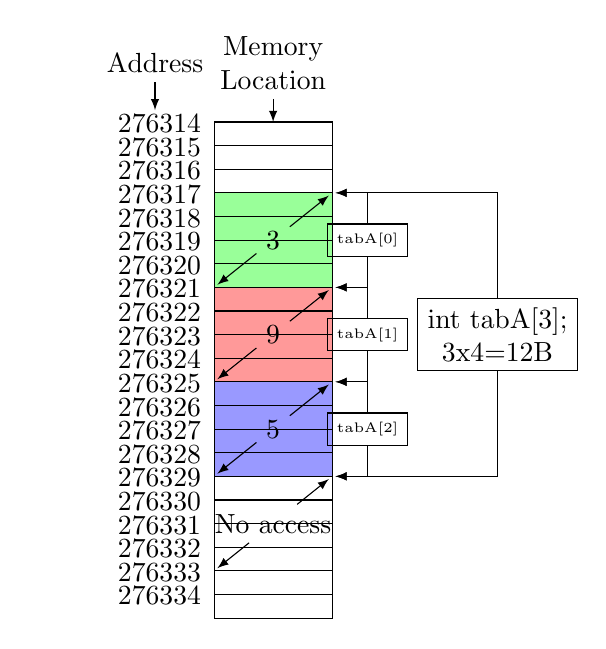
\begin{tikzpicture}[x=1.5cm,y=0.3cm]
  %% Building the boxes representing memory locations
  \foreach \x in {0,1,...,20}
  {
    \node[inner sep=1pt] (BL\x) at (0,-\x)   {};
    \node[inner sep=1pt] (UR\x) at (1,-\x+1) {};
    \node (MM\x) at ($(BL\x)!0.5!(UR\x)$) {};
    \draw (BL\x) rectangle (UR\x);
    \edef\memoryNumber{\number\numexpr276314+\x\relax}
    \node[anchor=south east] at (BL\x.north west) {\memoryNumber};
  }

  %% Label columns:
  \node (MEMLOC) at ($(MM0)+(0.0,0.9cm)$) { \parbox{2cm}{\centering Memory Location} };
  \node (ADDRESS) at ($(MEMLOC)-(1.0,0)$) {\parbox{3cm}{\centering Address} };
  \draw [-latex] (MEMLOC) -- ($(MM0|-UR0)+(0.0,0)$);
  \draw [-latex] (ADDRESS) -- ($(MM0|-UR0)-(1,-0.5)$);

  \foreach \x in {3,...,6}
  {
    \node[inner sep=1pt] (BL\x) at (0,-\x)   {};
    \node[inner sep=1pt] (UR\x) at (1,-\x+1) {};
    \node (MM\x) at ($(BL\x)!0.5!(UR\x)$) {};
    \draw[fill=green!40] (BL\x) rectangle (UR\x);
  }
  \foreach \x/\y in {7/3}
  {
    \node[draw] (M\x-\y) at ($0.5*(UR\x)+0.5*(UR\y)+(0.3,0)$)
    { {\centering \tiny tabA[0]}};
    \draw[-latex]  (M\x-\y) |- (UR\x) ; 
    \draw[-latex]  (M\x-\y) |- (UR\y) ;
  }
  \foreach \x/\y in {6/3}
  {
    \node (M\x-\y) at ($(BL\x)!0.5!(UR\y)$) {3};
    \draw[-latex]  (M\x-\y) -- (BL\x) ; 
    \draw[-latex]  (M\x-\y) -- (UR\y) ;
  }
  \foreach \x in {7,...,11}
  {
    \node[inner sep=1pt] (BL\x) at (0,-\x)   {};
    \node[inner sep=1pt] (UR\x) at (1,-\x+1) {};
    \node (MM\x) at ($(BL\x)!0.5!(UR\x)$) {};
    \draw[fill=red!40] (BL\x) rectangle (UR\x);
  }
  \foreach \x/\y in {11/7}
  {
    \node[draw] (M\x-\y) at ($0.5*(UR\x)+0.5*(UR\y)+(0.3,0)$)
    { {\centering \tiny tabA[1]}};
    \draw[-latex]  (M\x-\y) |- (UR\x) ; 
    \draw[-latex]  (M\x-\y) |- (UR\y) ;
  }
  \foreach \x/\y in {10/7}
  {
    \node (M\x-\y) at ($(BL\x)!0.5!(UR\y)$) {9};
    \draw[-latex]  (M\x-\y) -- (BL\x) ; 
    \draw[-latex]  (M\x-\y) -- (UR\y) ;
  }
  \foreach \x in {11,...,14}
  {
    \node[inner sep=1pt] (BL\x) at (0,-\x)   {};
    \node[inner sep=1pt] (UR\x) at (1,-\x+1) {};
    \node (MM\x) at ($(BL\x)!0.5!(UR\x)$) {};
    \draw[fill=blue!40] (BL\x) rectangle (UR\x);
  }
  \foreach \x/\y in {15/11}
  {
    \node[draw] (M\x-\y) at ($0.5*(UR\x)+0.5*(UR\y)+(0.3,0)$)
    { {\centering \tiny tabA[2]}};
    \draw[-latex]  (M\x-\y) |- (UR\x) ; 
    \draw[-latex]  (M\x-\y) |- (UR\y) ;
  }
  \foreach \x/\y in {14/11}
  {
    \node (M\x-\y) at ($(BL\x)!0.5!(UR\y)$) {5};
    \draw[-latex]  (M\x-\y) -- (BL\x) ; 
    \draw[-latex]  (M\x-\y) -- (UR\y) ;
  }
  \foreach \x/\y in {18/15}
  {
    \node (M\x-\y) at ($(BL\x)!0.5!(UR\y)$) {No access};
    \draw[-latex]  (M\x-\y) -- (BL\x) ; 
    \draw[-latex]  (M\x-\y) -- (UR\y) ;
  }
  
  \foreach \x/\y in {15/3}
  {
    \node[draw] (M\x-\y) at ($0.5*(UR\x)+0.5*(UR\y)+(1.4,0)$)
    { \parbox{1.8cm}{\centering int tabA[3];\\3x4=12B}};
    \draw[-latex]  (M\x-\y) |- (UR\x) ; 
    \draw[-latex]  (M\x-\y) |- (UR\y) ;
  }


\end{tikzpicture}
    \end{column}
    \begin{column}{0.5\textwidth}
\begin{itemize}
  \item Acces elements with [ ]
  \item Elements are indexed from 0
  \item Last element is \textit{size-1}
  \item Must make sure not to acces out of bounds
\end{itemize}

\begin{lstlisting}
int tabA[3];
tabA[0] = 3;
tabA[1] = 9;
tabA[2] = 5;
\end{lstlisting}
\begin{itemize}
  \item Out of bounds access:
\end{itemize}
\begin{lstlisting}
tabA[3]=0; //Error!!
\end{lstlisting}

    \end{column}
  \end{columns}
\end{frame}

\begin{frame}[fragile]
  \frametitle{1D arrays}
  \framesubtitle{Arrays are pointers}
  \vspace{-0.3cm}
  \begin{columns}
    \begin{column}{0.65\textwidth}
      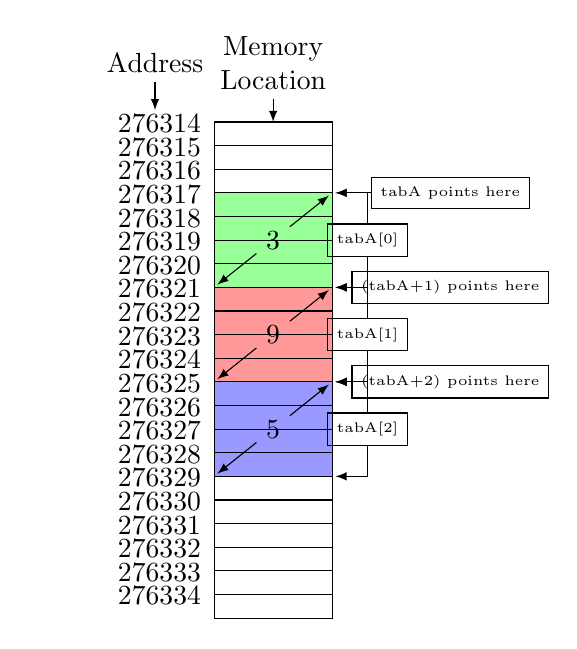
\begin{tikzpicture}[x=1.5cm,y=0.3cm]
  %% Building the boxes representing memory locations
  \foreach \x in {0,1,...,20}
  {
    \node[inner sep=1pt] (BL\x) at (0,-\x)   {};
    \node[inner sep=1pt] (UR\x) at (1,-\x+1) {};
    \node (MM\x) at ($(BL\x)!0.5!(UR\x)$) {};
    \draw (BL\x) rectangle (UR\x);
    \edef\memoryNumber{\number\numexpr276314+\x\relax}
    \node[anchor=south east] at (BL\x.north west) {\memoryNumber};
  }

  %% Label columns:
  \node (MEMLOC) at ($(MM0)+(0.0,0.9cm)$) { \parbox{2cm}{\centering Memory Location} };
  \node (ADDRESS) at ($(MEMLOC)-(1.0,0)$) {\parbox{3cm}{\centering Address} };
  \draw [-latex] (MEMLOC) -- ($(MM0|-UR0)+(0.0,0)$);
  \draw [-latex] (ADDRESS) -- ($(MM0|-UR0)-(1,-0.5)$);

  \foreach \x in {3,...,6}
  {
    \node[inner sep=1pt] (BL\x) at (0,-\x)   {};
    \node[inner sep=1pt] (UR\x) at (1,-\x+1) {};
    \node (MM\x) at ($(BL\x)!0.5!(UR\x)$) {};
    \draw[fill=green!40] (BL\x) rectangle (UR\x);
  }
  \foreach \x/\y in {7/3}
  {
    \node[draw] (M\x-\y) at ($0.5*(UR\x)+0.5*(UR\y)+(0.3,0)$)
    { {\centering \tiny tabA[0]}};
    \draw[-latex]  (M\x-\y) |- (UR\x) ; 
    \draw[-latex]  (M\x-\y) |- (UR\y) ;
  }
  \node[draw] (a) at ($(UR3)+(1,0)$){{\tiny tabA points here}};
  \draw[-latex]  (a) -- (UR3);
  \foreach \x/\y in {6/3}
  {
    \node (M\x-\y) at ($(BL\x)!0.5!(UR\y)$) {3};
    \draw[-latex]  (M\x-\y) -- (BL\x) ; 
    \draw[-latex]  (M\x-\y) -- (UR\y) ;
  }
  \foreach \x in {7,...,11}
  {
    \node[inner sep=1pt] (BL\x) at (0,-\x)   {};
    \node[inner sep=1pt] (UR\x) at (1,-\x+1) {};
    \node (MM\x) at ($(BL\x)!0.5!(UR\x)$) {};
    \draw[fill=red!40] (BL\x) rectangle (UR\x);
  }
  \foreach \x/\y in {11/7}
  {
    \node[draw] (M\x-\y) at ($0.5*(UR\x)+0.5*(UR\y)+(0.3,0)$)
    { {\centering \tiny tabA[1]}};
    \draw[-latex]  (M\x-\y) |- (UR\x) ; 
    \draw[-latex]  (M\x-\y) |- (UR\y) ;
  }
  \node[draw] (a) at ($(UR7)+(1,0)$){{\tiny (tabA+1) points here}};
  \draw[-latex]  (a) -- (UR7);
  \foreach \x/\y in {10/7}
  {
    \node (M\x-\y) at ($(BL\x)!0.5!(UR\y)$) {9};
    \draw[-latex]  (M\x-\y) -- (BL\x) ; 
    \draw[-latex]  (M\x-\y) -- (UR\y) ;
  }
  \foreach \x in {11,...,14}
  {
    \node[inner sep=1pt] (BL\x) at (0,-\x)   {};
    \node[inner sep=1pt] (UR\x) at (1,-\x+1) {};
    \node (MM\x) at ($(BL\x)!0.5!(UR\x)$) {};
    \draw[fill=blue!40] (BL\x) rectangle (UR\x);
  }
  \foreach \x/\y in {15/11}
  {
    \node[draw] (M\x-\y) at ($0.5*(UR\x)+0.5*(UR\y)+(0.3,0)$)
    { {\centering \tiny tabA[2]}};
    \draw[-latex]  (M\x-\y) |- (UR\x) ; 
    \draw[-latex]  (M\x-\y) |- (UR\y) ;
  }
  \node[draw] (a) at ($(UR11)+(1,0)$){{\tiny (tabA+2) points here}};
  \draw[-latex]  (a) -- (UR11);
  \foreach \x/\y in {14/11}
  {
    \node (M\x-\y) at ($(BL\x)!0.5!(UR\y)$) {5};
    \draw[-latex]  (M\x-\y) -- (BL\x) ; 
    \draw[-latex]  (M\x-\y) -- (UR\y) ;
  }

\end{tikzpicture}
    \end{column}
    \begin{column}{0.5\textwidth}
    \begin{itemize}
      \item Arrays are pointers
      \item \textit{tabA} points at the beginning of the array
      \item \&tabA[0] is equivalent to tabA
      \item pointer arithmetic applies
      \item (+ means +4B for int)
      \item * works
    \end{itemize}
\begin{lstlisting}
int tabA[3];
int *p=tabA;// no &
*p;//same as tabA[0]
*(p+1)//same as tabA[1]
*(p+2)//same as tabA[2]
\end{lstlisting}
\begin{itemize}
  \item There are some consequences ...
\end{itemize}
    \end{column}
  \end{columns}
\end{frame}

\begin{frame}[fragile]
  \frametitle{Passing arrays to functions}
Syntax:
\begin{lstlisting}
function_type function_name(array_type local_name[], int array_size)
\end{lstlisting}

e.g.:
\begin{lstlisting}
void FillArray(int A[], int n)
{
  for(int i=0; i<n; ++i)
    A[i]=i;
}
\end{lstlisting}

\end{frame}

\section{Random numbers}

\begin{frame}[fragile]
  \frametitle{Random numbers}
\begin{lstlisting}
#include <stdlib.h> //for random
#include <time.h> // for time

int my_random_number = rand();
//returns a number from a pseudo random sequence
//from 0 to RAND_MAX

srand(4);
//initialize the pseudo random sequence at some position

//use system time, to get different results at each run
//more rendomness
srand(time(NULL));
\end{lstlisting}

\end{frame}

\section{Sorting}

\begin{frame}
  \frametitle{Sorting}
  \framesubtitle{bubble sort}
  \begin{columns}
    \begin{column}{0.6\textwidth}
  \animategraphics[loop,autoplay,width=\textwidth,poster=first]{5}{something-}{0}{266}
    \end{column}
    \begin{column}{0.5\textwidth}
\begin{itemize}
  \item Simple sorting algorithm
  \item Compares pairs of elements, going through the collection
  \item easy implementation
  \item slow and impractical
  \item Complexity - cost, number of operations
  \item Worst $\sim n^2$ $O(n^2)$
  \item Best $\sim n$ $O(n)$
  \item There are better!
\end{itemize}
    \end{column}
  \end{columns}

\end{frame}

\begin{frame}[fragile]
  \frametitle{Bubble sort}
\begin{lstlisting}
void bubble_sort(int list[], int n)
{
  int c, d, t;
 
  for (c = 0 ; c < ( n - 1 ); c++)
  {
    for (d = 0 ; d < n - c - 1; d++)
    {
      if (list[d] > list[d+1])
      {
        t         = list[d];
        list[d]   = list[d+1];
        list[d+1] = t;
      }
    }
  }
}
\end{lstlisting}
\end{frame}

\section{Files}

\begin{frame}[fragile]
  \frametitle{Files}
FILE structure to handle files:
\begin{lstlisting}
FILE *fp;
\end{lstlisting}

To open a file use \textit{fopen()}:
\begin{lstlisting}
FILE *fopen(const char *filename, const char *mode);
//e.g.:
fp=fopen("c:\\test.txt", "r");
\end{lstlisting}

To close a file use \textit{fclose()}:
\begin{lstlisting}
int fclose(FILE *a_file);
//e.g.:
fclose(fp);
\end{lstlisting}
 
\end{frame}

\begin{frame}[fragile]
  \frametitle{Files}
  \framesubtitle{fopen modes}
  Depending on what we require the file to:
\begin{itemize}
	\item r  - open for reading
	\item w  - open for writing (file need not exist)
	\item a  - open for appending (file need not exist)
	\item r+ - open for reading and writing, start at beginning
	\item w+ - open for reading and writing (overwrite file)
	\item a+ - open for reading and writing (append if file exists)
\end{itemize}



\end{frame}

\begin{frame}[fragile]
  \frametitle{Files}
  \framesubtitle{Reading and writing with fprintf, fscanf}
Printing to file:
\begin{lstlisting}
FILE *fp;
fp=fopen("c:\\test.txt", "w");
fprintf(fp, "Testing...\n");

...
fclose(fp);
\end{lstlisting}

Reading from file:
\begin{lstlisting}
FILE *fp;
fp=fopen("c:\\test.txt", "w");
int a;
fcanf(fp, "%d", &a);
...
fclose(fp);
\end{lstlisting}
 
\end{frame}

\subsection{Examples}

\begin{frame}
  Use static arrays only.
  \frametitle{Examples}
  \begin{enumerate}
  \item Write a program that writes to a file coordinates to plot $f(x)=sin(x)$
for a range $<0,2\pi>$
  \item Write program that reads points coordinates from a file and decides if those are in a circle of radius 1.
  \item Write a program that generates N random numbers and stores them to a file.
  \item Write a program that reads a data file, calculates an average value and finds the number of elements above, and below that average.
  \item Write a program that reads values from a file, sorts them and stores them to a new file.
  \item Example test questions
\end{enumerate}
  
\end{frame}




\end{document}
